% Coefficient residues in O/(2), grouped by their image in O/P.
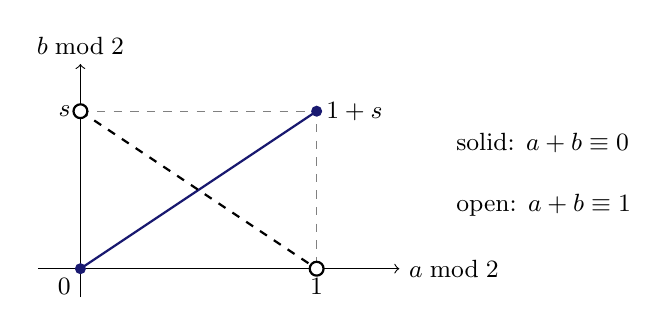
\begin{tikzpicture}[x=3cm,y=2cm,font=\small]
  \draw[->] (-.18,0)--(1.35,0) node[right] {$a\bmod2$};
  \draw[->] (0,-.18)--(0,1.3) node[above] {$b\bmod2$};
  \draw[dashed,gray] (0,1)--(1,1)--(1,0);
  \draw[thick,MidnightBlue] (0,0)--(1,1);
  \draw[thick,dashed] (0,1)--(1,0);
  \fill[MidnightBlue] (0,0) circle(2pt);
  \fill[MidnightBlue] (1,1) circle(2pt);
  \draw[fill=white,thick] (0,1) circle(2.5pt);
  \draw[fill=white,thick] (1,0) circle(2.5pt);
  \node[below left] at (0,0) {$0$};
  \node[below] at (1,0) {$1$};
  \node[left] at (0,1) {$s$};
  \node[right] at (1,1) {$1+s$};
  \node[anchor=west] at (1.55,.8) {solid: $a+b\equiv0$};
  \node[anchor=west] at (1.55,.4) {open: $a+b\equiv1$};
\end{tikzpicture}
